\documentclass{article}
\usepackage[margin=2.5cm, top=4cm, headheight=25pt]{geometry}
\usepackage{amsmath, amssymb, enumitem, fancyhdr, graphicx}
\usepackage[indent=20pt]{parskip}
\usepackage[hidelinks]{hyperref}
\usepackage{xcolor}
\usepackage{listings}
\usepackage{subcaption}
\usepackage{url}
\usepackage[most]{tcolorbox}
\usepackage{lastpage}
\usepackage{tikz}
\usepackage{circuitikz}

\usetikzlibrary{arrows, positioning}
\tcbuselibrary{listingsutf8} % Support for lstlistings within tcolorbox

\newtcolorbox[auto counter, number within=section]{question}[1][]{%
    colframe=gray!80,                      % Dark gray frame
    colback=gray!5,                       % Light gray background
    coltitle=black,                        % Black title
    title=\textbf{Question~\thetcbcounter}, % Bold title
    fonttitle=\bfseries\large,             % Subtle title font size
    rounded corners,                   % Slightly more rounded corners
    boxrule=0.25mm,                         % Thinner border for a sleek look
    enhanced,                              % Enhanced box features
    attach boxed title to top left={xshift=2mm, yshift=-2mm},
    boxed title style={colframe=gray!80, colback=gray!5, boxrule=0.25mm},
    % Title styling
    #1
}

\bibliographystyle{IEEEtran}
\graphicspath{{./images/}}

% -- Custom Variables --
\def\me{Rajdeep Gill 7934493}
\def\course{ECE 3760}
\def\labsection{A01}

\def\labno{10}
\def\title{Assignment 10: Message Sequence Chart}

% -- Styling for code snippets --
\lstset{
    basicstyle=\ttfamily\scriptsize,           % Basic font style
    keywordstyle=\color{blue},            % Keywords color
    commentstyle=\color{gray},            % Comments color
    stringstyle=\color{teal},             % Strings color
    numbers=left,                         % Line numbers on the left
    numberstyle=\tiny\color{gray},        % Line number style
    stepnumber=1,                         % Line number step
    numbersep=10pt,                       % Space between line numbers and code
    backgroundcolor=\color{lightgray!10}, % Background color
    frame=single,                         % Adds a frame around the code
    breaklines=true,                      % Line breaking for long lines
    captionpos=b,                         % Caption position
    showspaces=false,                     % Don't show spaces
    showstringspaces=false                % Don't show spaces in strings
}
\renewcommand{\lstlistingname}{Code Snippet}

\renewcommand{\arraystretch}{1.2} % For less-ugly tables
\setlength\parindent{0pt}

%----- Samples 
% Questions:
%   \begin{question}[title=Custom Question Title]
%       Question details
%   \end{question}

% Tables:
%   \begin{table}[htbp]
%       \centering
%       \caption{Table Caption}
%       \begin{tabular}{ll}
%           \toprule
%           \textbf{Column 1} & \textbf{Column 2} \\
%           \midrule
%           Row 1 & Row 2 \\
%           Row 3 & Row 4 \\
%           \bottomrule
%       \end{tabular}
%   \end{table} 

% Figures:
%   Single figure:
%       \begin{figure}[htbp]
%           \centering
%           \includegraphics[width=0.5\textwidth]{example-image}
%           \caption{Figure Caption}
%       \end{figure}
%   Multiple figures:
%       \begin{figure}[htbp]
%           \centering
%           \begin{subfigure}[b]{0.5\textwidth}
%               \includegraphics[width=\textwidth]{example-image-a}
%               \caption{First subfigure}
%           \end{subfigure}
%           \begin{subfigure}[b]{0.5\textwidth}
%               \includegraphics[width=\textwidth]{example-image-b}
%               \caption{Second subfigure}
%           \end{subfigure}
%           \caption{Main figure}
%       \end{figure}

\begin{document}

% --------------------------------------------------------------------------------
% TITLE
% --------------------------------------------------------------------------------

\begin{center}
    \huge \title

    \vspace{2mm}
    \hrule

    \vspace{4mm}
    \large \me

    \vspace{2mm}
    \large \course~\labsection

    \vspace{2mm}
    \today
\end{center}

\vspace{4mm}

% --------------------------------------------------------------------------------
% END TITLE
% --------------------------------------------------------------------------------

\newpage


\vspace{1cm}
\newpage

\pagestyle{fancy}
\fancyhead[L]{\large Assignment \labno}
\fancyhead[R]{\large \me}

\fancyfoot[C]{Page \thepage~of~\pageref{LastPage}}

% --------------------------------------------------------------------------------
% BODY
% --------------------------------------------------------------------------------

\section{Message Sequence Chart}

\autoref{fig:msgchart} shows the message sequence chart for a skip sending some commands. The skip first sends a sweep hard command, which changes the LEDs on both sweeper devices. The sweeper's then interpret the LED pattern and perform the proper action. The skip then sends a clean command followed by a stop command.

\begin{figure}[ht!]
    \centering
    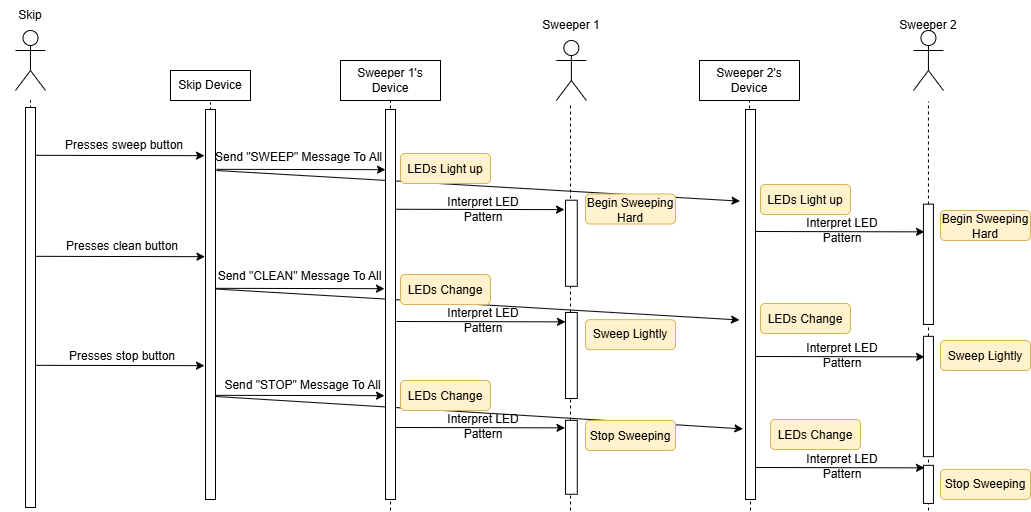
\includegraphics[width=0.75\textwidth]{Message Sequence Diagram-2.png}
    \caption{Message Sequence Chart}
    \label{fig:msgchart}
\end{figure}

This illustrates 3 of the 5 commands. With the other 2 commands, a similar sequence would be followed, the skip presses a button, the sweeper device lights up, and the sweeper interprets the command and performs the proper action. There is no feedback from the sweeper device thus the skip does not need to wait for a response before sending the next command.

\textbf{Approval:}

Since ESP-NOW operates on the same frequency as WiFi, regulatory approval may be required if this device is intended for sale. In the U.S., the device would need FCC approval, while in Canada, certification from ISED would be necessary. Given its low power consumption, it would likely qualify as license-exempt, but testing is required to confirm compliance.

Further research is needed, but the ISED website outlines various certification requirements. Key regulatory standards include RSS-210\footnote{\url{https://ised-isde.canada.ca/site/spectrum-management-telecommunications/en/devices-and-equipment/radio-equipment-standards/radio-standards-specifications-rss/rss-210-licence-exempt-radio-apparatus-category-i-equipment}}, RSS-GEN\footnote{\url{https://ised-isde.canada.ca/site/spectrum-management-telecommunications/en/devices-and-equipment/radio-equipment-standards/radio-standards-specifications-rss/rss-210-licence-exempt-radio-apparatus-category-i-equipment}}, and RSS-247\footnote{\url{https://ised-isde.canada.ca/site/spectrum-management-telecommunications/en/devices-and-equipment/radio-equipment-standards/radio-standards-specifications-rss/rss-247-digital-transmission-systems-dtss-frequency-hopping-systems-fhss-and-licence-exempt-local}}.



% --------------------------------------------------------------------------------
% END BODY
% --------------------------------------------------------------------------------

\end{document}
